\chapter{Introdução}

A robótica é um ramo da tecnologia que lida com a concepção, construção,
operação e aplicação de máquinas capazes de realizar uma série de ações de
maneira autônoma.  Atualmente é um tópico em rápida ascensão.  Pesquisar,
projetar e fabricar novos robôs serve vários propósitos práticos tais como
domésticos, comerciais e militares.  Um dos problemas atuas da robótica é o
planejamento em ambientes multi-agentes dinâmicos e competitivos.  Um exemplo de
um problema dessa classe é um jogo de futebol de robôs, onde um grupo de robôs é
controlado por uma IA independente.  A Figura~\ref{fig:robocup2013} mostra uma
imagem da Robocup 2013, competição internacional de robótica, onde a equipe
RoboIME (de alunos do Laboratório de Robótica do IME) participou.

\begin{figure}[h]
  \centering
  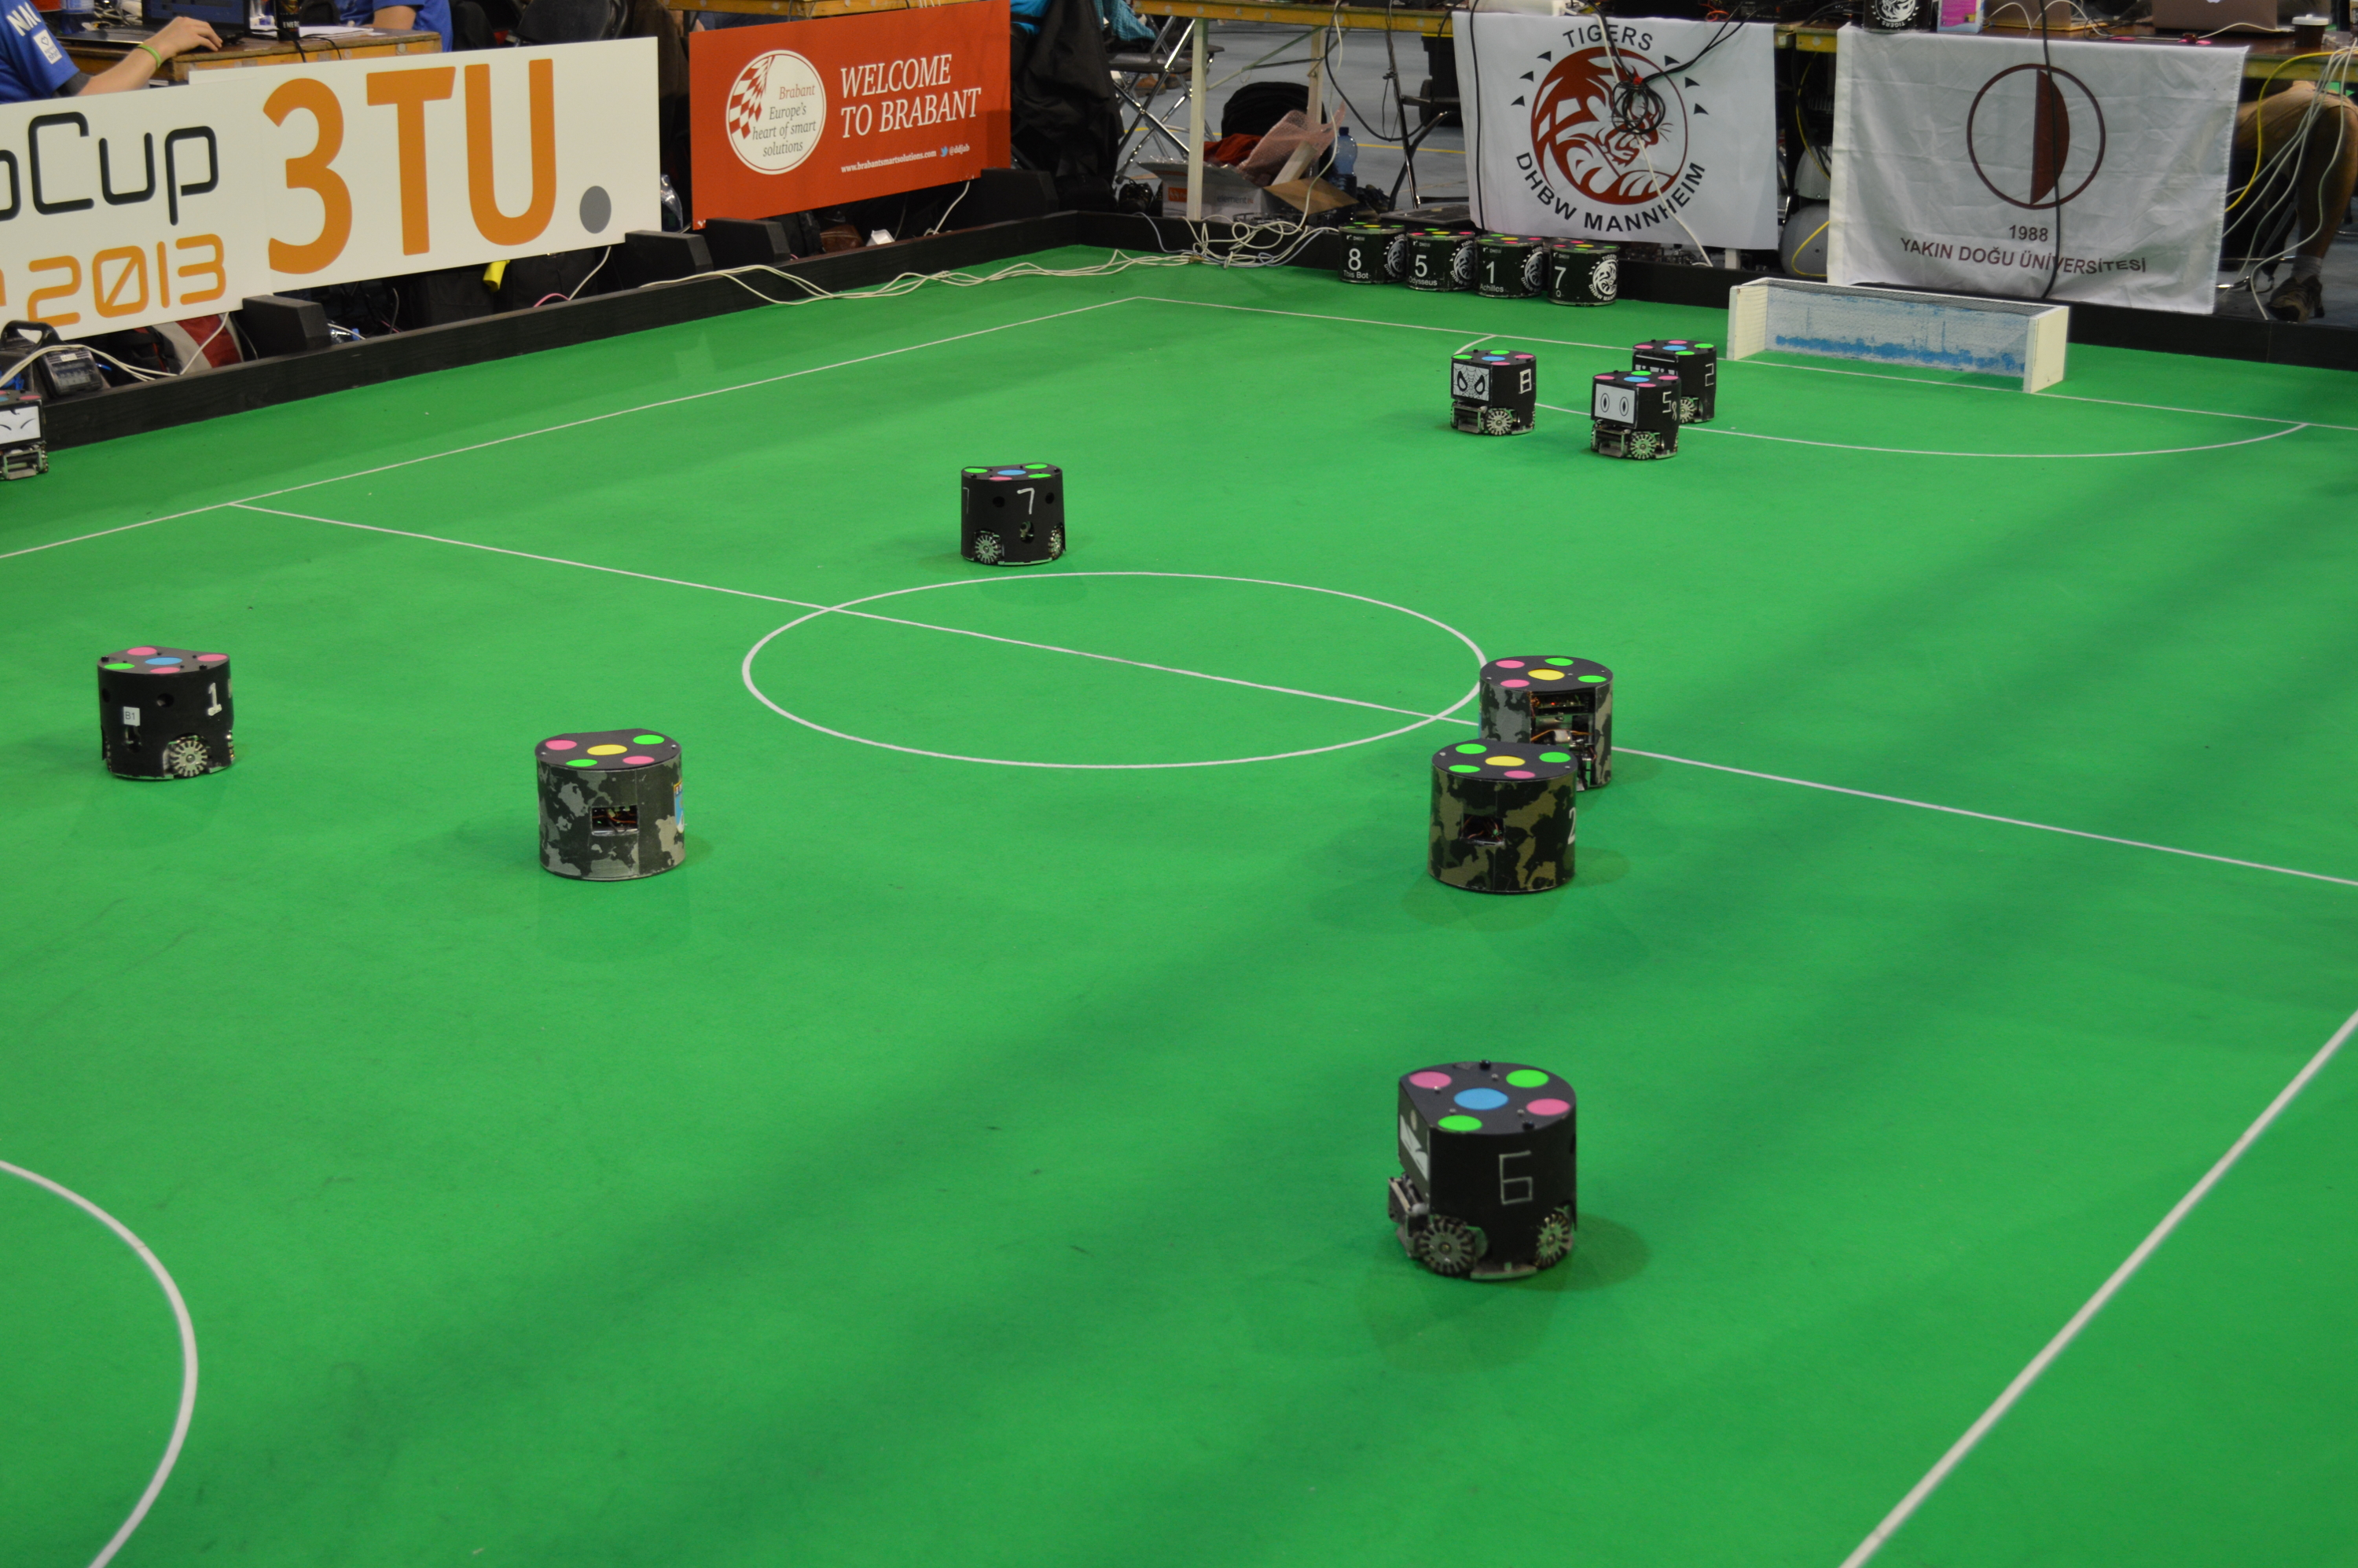
\includegraphics[width=0.8\linewidth]{robocup2013}
  \caption{Imagem da SSL \textit{RoboCup} 2013 em Eindhoven, na Holanda}\label{fig:robocup2013}
\end{figure}

Devido a alta complexidade desses ambientes, não é viável o planejamento
considerando diretamente as leis físicas.  Como consequência, limita-se as ações
possíveis do robô no modelo utilizado no planejamento para que se possa simular
mais situações em tempo hábil, uma vez que o ambiente está continuamente sujeito
a modificações.  Entretanto, para que as simulações sejam válidas, o robô real
deve estar em sintonia com seu modelo.  Com efeito, o robô real deve executar os
comandos conforme o robô simulado, caso o mesmo ambiente simulado seja
encontrado na prática.

A ideia de robôs jogando futebol foi mencionada pela primeira vez pelo professor
Alan Mackworth (University of British Columbia, Canadá) em um artigo intitulado
"On Seeing Robots", apresentado no Vision Interface 92 e posteriormente
publicado em um livro chamado Computer Vision: System, Theory and Applications
\cite{basu1993computer}.  Independentemente, um grupo de pesquisadores japoneses
organizou um Workshop no Ground Challenge in Artificial Intelligence, em Outubro
de 1992, Tóquio, discutindo e propondo problemas que representavam grandes
desafios.  Esse Workshop os levou a sérias discussões sobre usar um jogo de
futebol para promover ciência e tecnologia.  Estudos foram feitos para analisar
a viabilidade dessa ideia.  Os resultados desses estudos mostram que a ideia era
viável, desejável e englobava diversas aplicações práticas.  Em 1993, um grupo
de pesquisadores, incluindo Minoru Asada, Yasuo Kuniyoshi e Hiroaki Kitano,
lançaram uma competição de robótica chamada de Robot J-League (fazendo uma
analogia à J-League, nome da Liga Japonesa de Futebol Profissional).  Em um mês,
vários pesquisadores já se pronunciavam dizendo que a iniciativa deveria ser
estendida ao âmbito internacional.  Surgia então, a Robot World Cup Initiative
(RoboCup).

RoboCup é uma competição destinada a desenvolver os estudos na área de robótica
e Inteligência Artificial (IA) por meio de uma competição amigável.  Além disso,
ela tem como objetivo, até 2050, desenvolver uma equipe de robôs humanoides
totalmente autônomos capazes de derrotar a equipe campeã mundial de futebol
humano.  A competição possui várias modalidades.  Neste trabalho, será analisada
a Small Size Robot League (SSL), também conhecida como F180.  De acordo com as
regras da SSL de 2015, as equipes devem ser compostas por 6 robôs, sendo um
deles o goleiro, que deve ser designado antes do início do jogo.  Durante o
jogo, nenhuma interferência humana é permitida com o sistema de controle dos
robôs.  É fornecido aos times um sistema de visão global e esses controlam seus
robôs através de máquinas próprias.  O sistema de controle dos robôs geralmente
é externo e recebe os dados de um conjunto de duas câmeras localizadas acima do
campo.  Esse sistema de controle processa os dados, determina qual comando deve
ser executado por cada robô e envia este comando através de ondas de rádio aos
robôs.
% Embora seja permitido que as equipes utilizem sistemas próprios de visão, a
% maioria das equipes utiliza a visão centralizada.

\section{Motivação}

% TODO: ABRIR AQUI UMA SUBSEÇÃO DENOMINADA CONTEXTUALIZAÇÃO INICIAL E COLOCAR AS
%       SEÇÕES 2.1 E 2.2 CO IP COMO SUBITENS. ?????

O futebol de robôs, problema padrão de investigação internacional, reúne grande
parte dos desafios presentes em problemas do mundo real a serem resolvidos em
tempo real.  As soluções encontradas para o futebol de robôs podem ser
estendidas, possibilitando o uso da robótica em locais de difícil acesso para
humanos, ambientes insalubres e situações de risco de vida iminente.  Há
diversas novas áreas de aplicação da robótica, tais como exploração espacial e
submarina, navegação em ambientes inóspitos e perigosos, serviço de assistência
médica e cirúrgica, além do setor de entretenimento.  Essas áreas podem ser
beneficiadas com o desenvolvimento de sistemas multi robôs.  Nestes domínios de
aplicação, sistemas de multi robôs deparam-se sempre com tarefas muito difíceis
de serem efetuadas por um único robô.  Um time de robôs pode prover redundância
e contribuir cooperativamente para resolver o problema em questão.  Com efeito,
eles podem resolver o problema de maneira mais confiável, mais rápida e mais
econômica, quando comparado com o desempenho que único robô teria.

Devido a alta complexidade de sistemas multi-agentes dinâmicos, torna-se
necessário um modelo simplificado para que sejam executadas o maior número de
simulações possível.  Caso seja possível uma discretização, ter-se-á um número
finito de casos para serem avaliados.  Com isso, pode-se desenvolver um sistema
multi-agente baseado em utilidade.  Assim, o computador passa a escolher parte
da estratégia com base na função utilidade escolhida.
%como o Minimax (discutido no Capítulo~\ref{cap:minimax}) para encontrar
%soluções ao problema.

Isso é mais desejável que um modelo heurístico de IA, onde as soluções são
criadas com base nos ambientes identificados pelos modeladores.  Isso, pois a
modelagem puramente heurística limita o número de jogadas que se pode executar e
limita a capacidade que o computador tem de testar um grande número de
possibilidades.  O resultado é que a qualidade das jogadas se limita a
capacidade de quem cria as heurísticas.

\section{Objetivo}

O objetivo deste trabalho é desenvolver uma ferramenta de representação
comportamental baseado em otimização para futebol de robôs.
%O objetivo deste trabalho é desenvolver um algoritmo de controle para o futebol
%de robôs que obtenha um desempenho melhor que o utilizado atualmente, de acordo
%com a performance em um conjunto de partidas.
A meta intermediária é criar um modelo discreto sequencial para o problema do
futebol de robôs.  A partir desta discretização, foi desenvolvida uma arquitetura
de controle que seleciona jogadas o mais próximas da jogada ótima possível, de
acordo com uma função de avaliação e dentro do tempo disponível para o
planejamento.

\section{Justificativa}
% TODO: incluir referências

Uma arquitetura de controle que simule os diversos ambientes dinamicamente de
maneira sequencial de um ambiente multi-agente permite que várias jogadas sejam
criadas dinamicamente, diferentemente de uma arquitetura estática baseada
somente em heurística.  Essa abordagem heurística tem origem na maneira como
estratégias são planejadas nos times de futebol humano.

Com tal mecanismo é possível melhorar a IA em uso pela RoboIME para tomar
decisões que levem a resultados melhores e, como consequência, ganhar mais
partidas.  Nenhuma equipe atualmente esta seguindo esta abordagem, mas os
autores acreditam que essa é uma linha de pesquisa promissora, já que se utiliza
da capacidade que o computador tem de simular várias possibilidades em um curto
intervalo de tempo.

\section{Metodologia}

Para atingir os objetivos propostos foi seguida a seguinte metodologia.
O problema em questão foi modelado. A partir dessa modelagem, foi
criada uma função de avaliação para se avaliar as jogadas consideradas.
Com base nesse estudo, foi construída uma ferramenta para escolher
jogadas com base nessa função. Ao longo dos testes, foi necessário
ajusta a função citada, bem como o método de busca utilizado.

\section{Estrutura}

% modelagem
No Capítulo~\ref{cap:modelagem}, um modelo do futebol de robôs é proposto.
Também é apresentada a função de avaliação.

% arquitetura
No Capítulo~\ref{cap:arquitetura}, a ferramenta proposta é desenvolvida com
base no modelo proposto anteriormente.

% resultados
No Capítulo~\ref{cap:resultados}, são apresentados os resultados obtidos
neste trabalho.

% considerações finais
%No Capítulo~\ref{cap:cons_finais}, são apresentadas sugestões para trabalhos
%futuros e as principais dificuldades enfrentadas pelos autores são destacadas.

% conclusao
Finalmente, são apresentados os principais resultados atingidos neste trabalho.

% vim: tw=80 et ts=2 sw=2 sts=2 ft=tex
